\chapter{Etude Technique}

\section{Introduction}

Ce chapitre presente une etude technique detaillee de l'application d'analyse de sentiments basee sur une architecture de microservices moderne. L'architecture est conçue pour assurer une modularite, une evolutivite et une gestion efficace des services distribues. L'application comprend plusieurs composants principaux : un service FastAPI pour l'analyse de sentiments utilisant le modele cardiffnlp/twitter-xlm-roberta-base-sentiment \cite{10}, un frontend Next.js pour l'interface utilisateur, un service Spring Gateway pour la gestion des APIs, un service Keycloak pour l'authentification et l'autorisation, et un module Selenium pour le web scraping automatise des commentaires d'Hespress.

Cette etude couvre l'architecture des microservices, les technologies utilisees, les interactions entre les services et les choix de conception pour garantir une performance optimale dans le traitement et l'analyse des donnees textuelles en temps reel.

\section{Architecture des Microservices}

L'architecture de l'application d'analyse de sentiments est basee sur des microservices, où chaque service est conçu pour etre independant et interagir avec les autres services via des API bien definies. Cette section decrit l'architecture globale, les roles specifiques de chaque service, ainsi que les benefices qu'offre une architecture basee sur les microservices pour l'analyse de donnees textuelles.

\subsection{Description de l'Architecture}

L'architecture de notre projet d'analyse de sentiments est divisee en plusieurs services independants. Chaque service est responsable d'une fonctionnalite specifique et communique avec les autres services par le biais de protocoles de communication legers comme HTTP/REST. Cette approche permet une meilleure modularite, une scalabilite amelioree et une maintenance facilitee de l'application d'analyse.

Les services sont deployes de maniere independante, permettant une mise a l'echelle selective selon les besoins de charge de travail. Par exemple, le service d'analyse de sentiments peut etre scale independamment lors de pics d'analyse, tandis que le service de collecte peut fonctionner selon un planning predetermine.

\subsection{Architecture du Projet d'Analyse de Sentiments}

\begin{figure}[H]
\centering
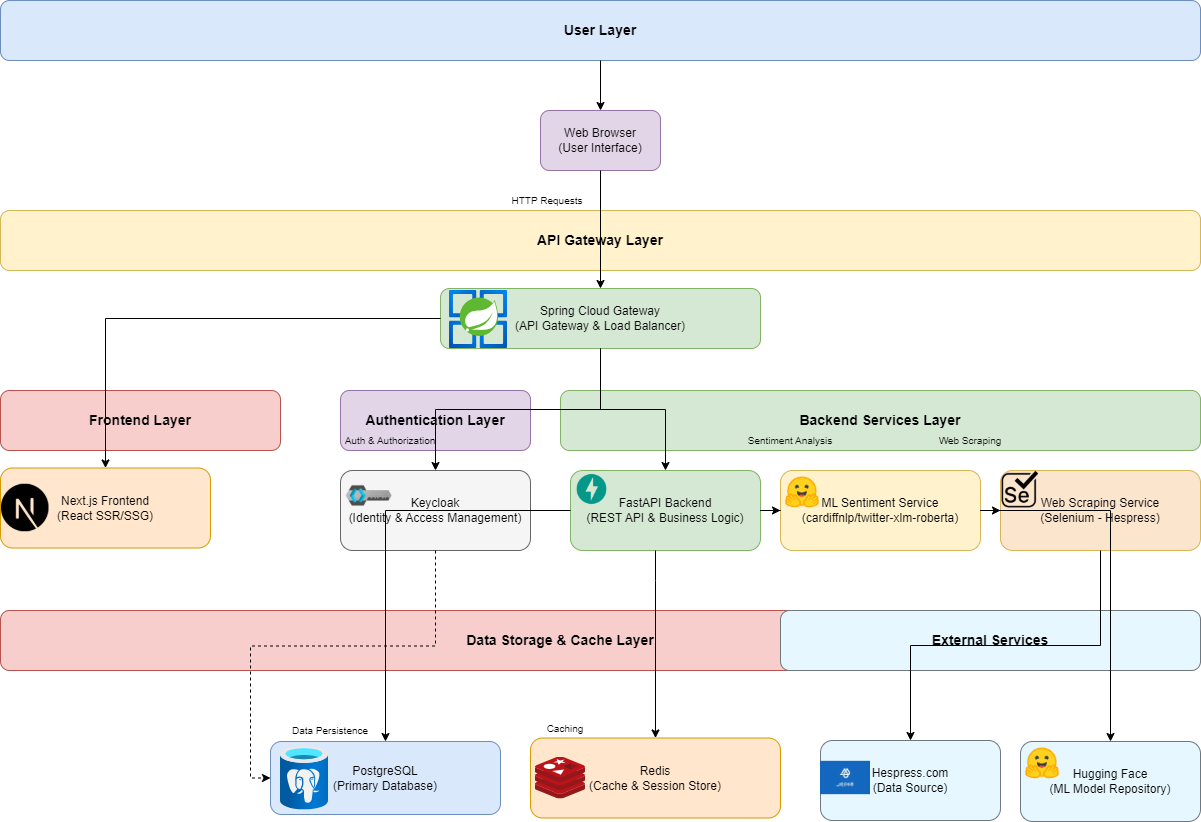
\includegraphics[height=14cm , width=\textwidth]{assets/images/arch.png}
\caption{Architecture globale du systeme d'analyse de sentiments}
\label{fig:architecture}
\end{figure}

\subsection{Description des Services}

\subsubsection{Service 1 : Frontend Next.js}

\textbf{Technologie} : Next.js, React, TypeScript

\textbf{Fonctionnalite} : Ce service fournit l'interface utilisateur moderne et reactive pour la visualisation des resultats d'analyse de sentiments. Il offre des tableaux de bord interactifs, des graphiques en temps reel et des outils de filtrage avances.

\textbf{Caracteristiques principales} :
\begin{itemize}
    \item Rendu cote serveur (SSR) pour des performances optimales
    \item Interface responsive adaptee aux differents appareils
    \item Composants interactifs pour la visualisation de donnees
    \item Integration avec l'API Gateway via des appels REST securises
\end{itemize}

\textbf{Endpoints principaux} :
\begin{itemize}
    \item \texttt{/dashboard} : Tableau de bord principal avec metriques
    \item \texttt{/analysis} : Interface d'analyse detaillee
    \item \texttt{/reports} : Generation et consultation de rapports
    \item \texttt{/settings} : Configuration utilisateur
\end{itemize}

\subsubsection{Service 2 : Backend d'Analyse - FastAPI}

\textbf{Technologie} : FastAPI, Python, Transformers (Hugging Face)

\textbf{Fonctionnalite} : Ce service est le cœur de l'application, responsable du traitement et de l'analyse des sentiments des commentaires collectes. Il utilise le modele pre-entraine cardiffnlp/twitter-xlm-roberta-base-sentiment \cite{10} pour classifier les sentiments en temps reel.

\textbf{Caracteristiques principales} :
\begin{itemize}
    \item Integration du modele XLM-RoBERTa pour l'analyse multilingue
    \item Traitement par lot pour l'analyse de gros volumes
    \item Cache Redis pour optimiser les performances
    \item API asynchrone pour un traitement non-bloquant
\end{itemize}

\textbf{Endpoints principaux} :
\begin{itemize}
    \item \texttt{POST /analyze/sentiment} : Analyse de sentiment d'un texte
    \item \texttt{POST /analyze/batch} : Analyse par lot de plusieurs textes
    \item \texttt{GET /analysis/results} : Recuperation des resultats d'analyse
    \item \texttt{GET /model/info} : Informations sur le modele utilise
\end{itemize}

\subsubsection{Service 3 : Collecte de Donnees - Selenium}

\textbf{Technologie} : Selenium WebDriver, Python, FastAPI

\textbf{Fonctionnalite} : Ce service automatise la collecte des commentaires sur le site Hespress en utilisant Selenium pour le web scraping. Il gere la navigation automatisee, l'extraction des donnees et la gestion des sessions.

\textbf{Caracteristiques principales} :
\begin{itemize}
    \item Scraping automatise et planifie
    \item Gestion des pages dynamiques avec JavaScript
    \item Rotation des User-Agents et gestion des timeouts
    \item Stockage structure des donnees collectees
\end{itemize}

\textbf{Endpoints principaux} :
\begin{itemize}
    \item \texttt{POST /scraping/start} : Demarrage de la collecte
    \item \texttt{GET /scraping/status} : Statut de la collecte en cours
    \item \texttt{GET /scraping/data} : Recuperation des donnees collectees
    \item \texttt{POST /scraping/config} : Configuration des parametres de collecte
\end{itemize}

\subsubsection{Service 4 : API Gateway - Spring Cloud Gateway}

\textbf{Technologie} : Spring Boot, Spring Cloud Gateway

\textbf{Fonctionnalite} : Ce service agit comme une passerelle unique pour tous les microservices, gerant le routage, la gestion des API, et servant de proxy pour les demandes des utilisateurs. Il centralise les appels aux microservices et offre des fonctionnalites telles que le load balancing, le rate limiting, et la securite.

\textbf{Caracteristiques principales} :
\begin{itemize}
    \item Routage intelligent vers les services appropries
    \item Load balancing et circuit breaker
    \item Limitation du taux de requetes (rate limiting)
    \item Logging centralise et monitoring
\end{itemize}

\textbf{Endpoints principaux} :
\begin{itemize}
    \item \texttt{/api/analysis/*} : Routes vers le service d'analyse
    \item \texttt{/api/scraping/*} : Routes vers le service de collecte
    \item \texttt{/api/auth/*} : Routes vers Keycloak
    \item \texttt{/actuator/*} : Endpoints de monitoring
\end{itemize}

\subsubsection{Service 5 : Authentification et Autorisation - Keycloak}

\textbf{Technologie} : Keycloak, OAuth 2.0, OpenID Connect

\textbf{Fonctionnalite} : Keycloak est utilise pour la gestion des identites et des acces, offrant des fonctionnalites telles que l'authentification, l'autorisation, la gestion des utilisateurs, et la federation des identites. Il securise les endpoints des autres microservices et gere les sessions utilisateurs.

\textbf{Caracteristiques principales} :
\begin{itemize}
    \item Authentification unique (SSO)
    \item Gestion granulaire des roles et permissions
    \item Integration OAuth 2.0 et OpenID Connect
    \item Interface d'administration pour la gestion des utilisateurs
\end{itemize}

\textbf{Endpoints principaux} :
\begin{itemize}
    \item \texttt{/auth/realms/sentiment/protocol/openid-connect/token} : Token d'authentification
    \item \texttt{/auth/admin/realms/sentiment/users} : Gestion des utilisateurs
    \item \texttt{/auth/realms/sentiment/protocol/openid-connect/userinfo} : Informations utilisateur
\end{itemize}

\section{Communication entre les Services}

La communication entre les microservices de l'application d'analyse de sentiments est principalement assuree via des API RESTful et des mecanismes de messaging asynchrone. Le service Spring Gateway agit comme un point d'entree unique pour toutes les requetes des utilisateurs et distribue ces requetes aux services appropries. Keycloak assure la securite des communications en authentifiant les utilisateurs et en autorisant les requetes.

\subsection{Communication via API RESTful}

Les API RESTful sont utilisees pour les interactions synchrones entre les microservices. Chaque service expose des endpoints specifiques pour recevoir et traiter les requetes, assurant ainsi une communication claire et structuree. Le Spring Gateway reçoit les requetes des utilisateurs, applique les regles de routage et transmet les requetes aux microservices correspondants.

\textbf{Flux de communication typique} :
\begin{enumerate}
    \item L'utilisateur envoie une requete via le frontend Next.js
    \item La requete passe par l'API Gateway qui verifie l'authentification
    \item L'API Gateway route la requete vers le service approprie (analyse ou collecte)
    \item Le service traite la requete et retourne la reponse
    \item La reponse remonte jusqu'au frontend pour affichage
\end{enumerate}

\subsection{Gestion des Donnees et Persistence}

Pour l'application d'analyse de sentiments, la gestion des donnees est cruciale car elle implique le stockage de grandes quantites de commentaires et de resultats d'analyse.

\textbf{Strategies de stockage} :
\begin{itemize}
    \item \textbf{Base de donnees relationnelle (PostgreSQL)} : Stockage des metadonnees, configurations et resultats d'analyse structures
    \item \textbf{Cache Redis} : Mise en cache des resultats d'analyse frequemment demandes pour optimiser les performances
    \item \textbf{Stockage de fichiers} : Sauvegarde des modeles entraines et des donnees brutes collectees
\end{itemize}

\subsection{Securite et Authentification}

La securite est implementee a plusieurs niveaux :

\begin{itemize}
    \item \textbf{Authentification} : Tokens JWT generes par Keycloak
    \item \textbf{Autorisation} : Verification des roles et permissions pour chaque endpoint
    \item \textbf{Communication securisee} : HTTPS pour toutes les communications externes
    \item \textbf{Validation des donnees} : Sanitisation des donnees collectees pour eviter les injections
\end{itemize}

\section{Technologies et Outils Utilises}

\subsection{Technologies Frontend}

\textbf{Next.js} : Framework React avec support SSR/SSG pour des performances optimales
\begin{itemize}
    \item Rendu hybride (statique et serveur)
    \item Optimisation automatique des images et du CSS
    \item Support TypeScript natif
    \item Hot reloading pour le developpement
\end{itemize}

\subsection{Technologies Backend}

\textbf{FastAPI} : Framework Python moderne pour la creation d'APIs hautes performances
\begin{itemize}
    \item Documentation automatique avec OpenAPI/Swagger
    \item Support asynchrone natif
    \item Validation automatique des donnees avec Pydantic
    \item Performance comparable a Node.js et Go
\end{itemize}

\textbf{Modele d'IA} : cardiffnlp/twitter-xlm-roberta-base-sentiment \cite{10}
\begin{itemize}
    \item Support multilingue (arabe, français, anglais)
    \item Optimise pour les textes courts (comme les commentaires)
    \item Precision elevee sur les taches de classification de sentiments
    \item Integration facile via Hugging Face Transformers
\end{itemize}

\subsection{Infrastructure et Deploiement}

\textbf{Docker} : Containerisation pour un deploiement consistent
\begin{itemize}
    \item Images legeres basees sur Alpine Linux
    \item Orchestration avec Docker Compose
    \item Isolation des services et dependances
\end{itemize}

\textbf{Monitoring et Logging} :
\begin{itemize}
    \item Logs centralises avec ELK Stack (Elasticsearch, Logstash, Kibana)
    \item Metriques de performance avec Prometheus et Grafana
    \item Health checks automatiques pour tous les services
\end{itemize}

\section{Choix de Conception et Justifications}

\subsection{Microservices vs Architecture Monolithique}

L'architecture microservices a ete choisie pour plusieurs raisons specifiques au projet d'analyse de sentiments :

\textbf{Avantages pour notre cas d'usage} :
\begin{itemize}
    \item \textbf{Scalabilite selective} : Le service d'analyse peut etre scale independamment lors de pics de charge
    \item \textbf{Technologies heterogenes} : Utilisation de Python pour l'IA et Java pour l'API Gateway selon les besoins
    \item \textbf{Deployment independant} : Mise a jour du modele d'IA sans affecter les autres services
    \item \textbf{Resilience} : Panne d'un service n'affecte pas l'ensemble du systeme
\end{itemize}

\subsection{Choix du Modele d'IA}

Le modele cardiffnlp/twitter-xlm-roberta-base-sentiment \cite{10} a ete selectionne pour :

\begin{itemize}
    \item \textbf{Support multilingue} : Capacite a traiter l'arabe, le français et la darija marocaine
    \item \textbf{Optimisation reseaux sociaux} : Entraine specifiquement sur des donnees Twitter similaires aux commentaires
    \item \textbf{Performance prouvee} : Resultats benchmarks superieurs sur les taches de sentiment analysis
    \item \textbf{Facilite d'integration} : Disponible via Hugging Face avec une API simple
\end{itemize}

\subsection{Securite avec Keycloak}

Keycloak est utilise pour securiser l'application d'analyse de sentiments car il offre :

\begin{itemize}
    \item \textbf{SSO (Single Sign-On)} : Authentification unique pour tous les services
    \item \textbf{Federation d'identites} : Integration possible avec des systemes existants
    \item \textbf{Gestion granulaire des permissions} : Controle d'acces par role et ressource
    \item \textbf{Standards modernes} : Support OAuth 2.0 et OpenID Connect
\end{itemize}

\subsection{Performance et Optimisation}

Plusieurs strategies d'optimisation ont ete implementees :

\begin{itemize}
    \item \textbf{Cache Redis} : Mise en cache des resultats d'analyse pour eviter les recalculs
    \item \textbf{Traitement par lot} : Analyse de plusieurs commentaires simultanement
    \item \textbf{Lazy loading} : Chargement du modele uniquement quand necessaire
    \item \textbf{Connection pooling} : Reutilisation des connexions base de donnees
\end{itemize}

\section{Diagrammes de Sequence}

\subsection{Processus d'Analyse de Sentiments}

\begin{landscape}
\begin{figure}[H]
\centering
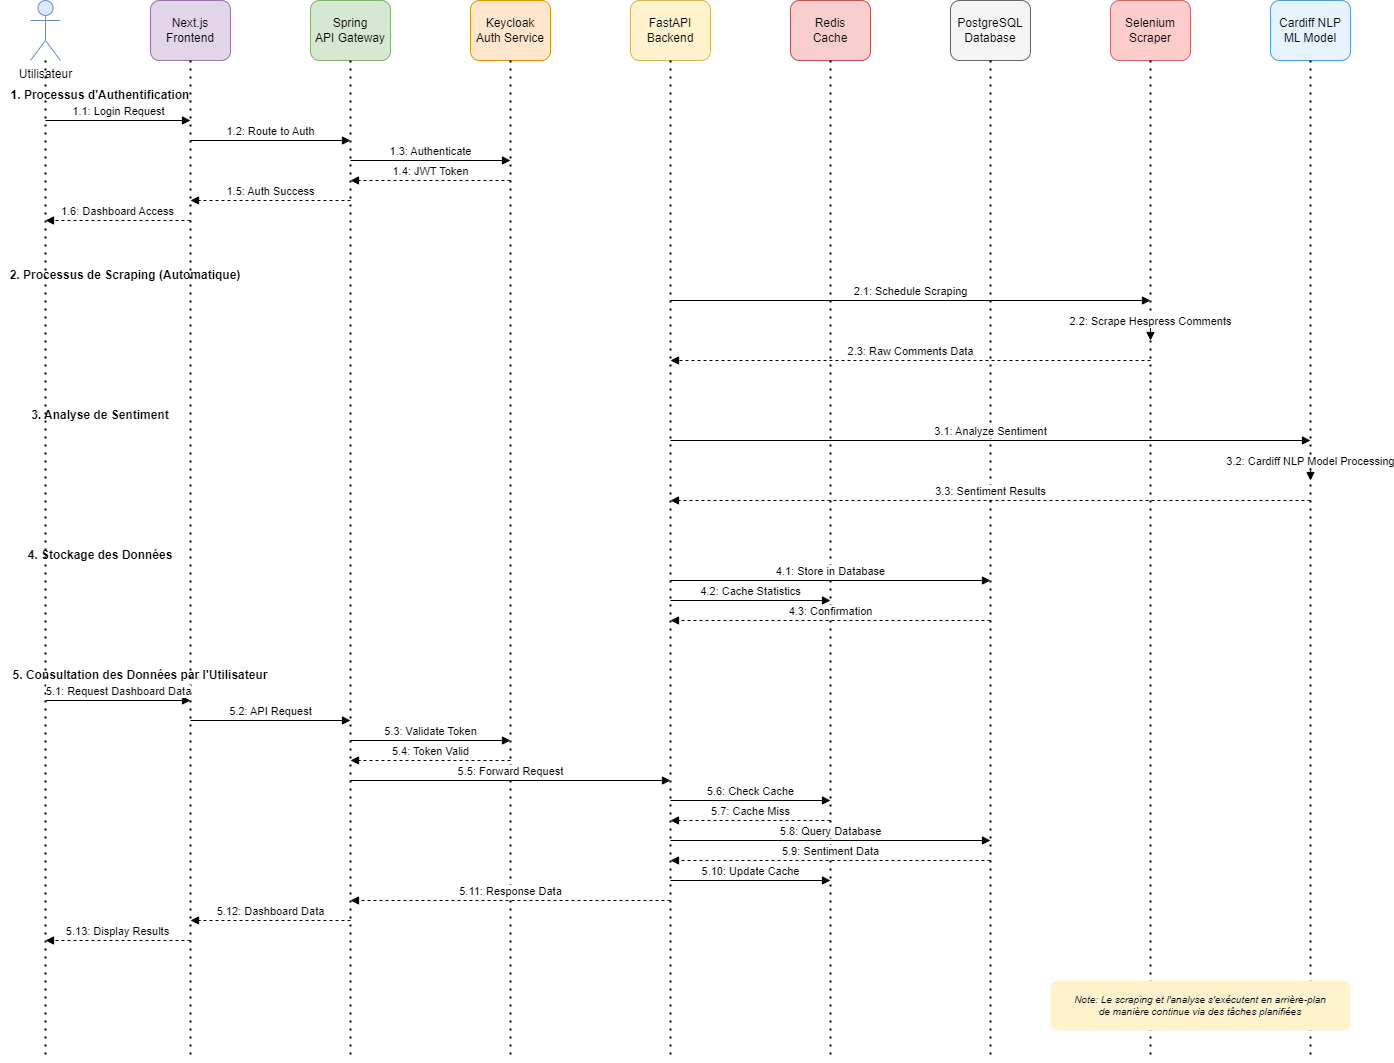
\includegraphics[ width=19 cm]{assets/images/sequence.png}
\caption{Diagramme de sequence pour l'analyse de sentiments}
\label{fig:seq-analysis}
\end{figure}
\end{landscape}

\subsection{Processus d'Authentification}

\begin{figure}[H]
\centering
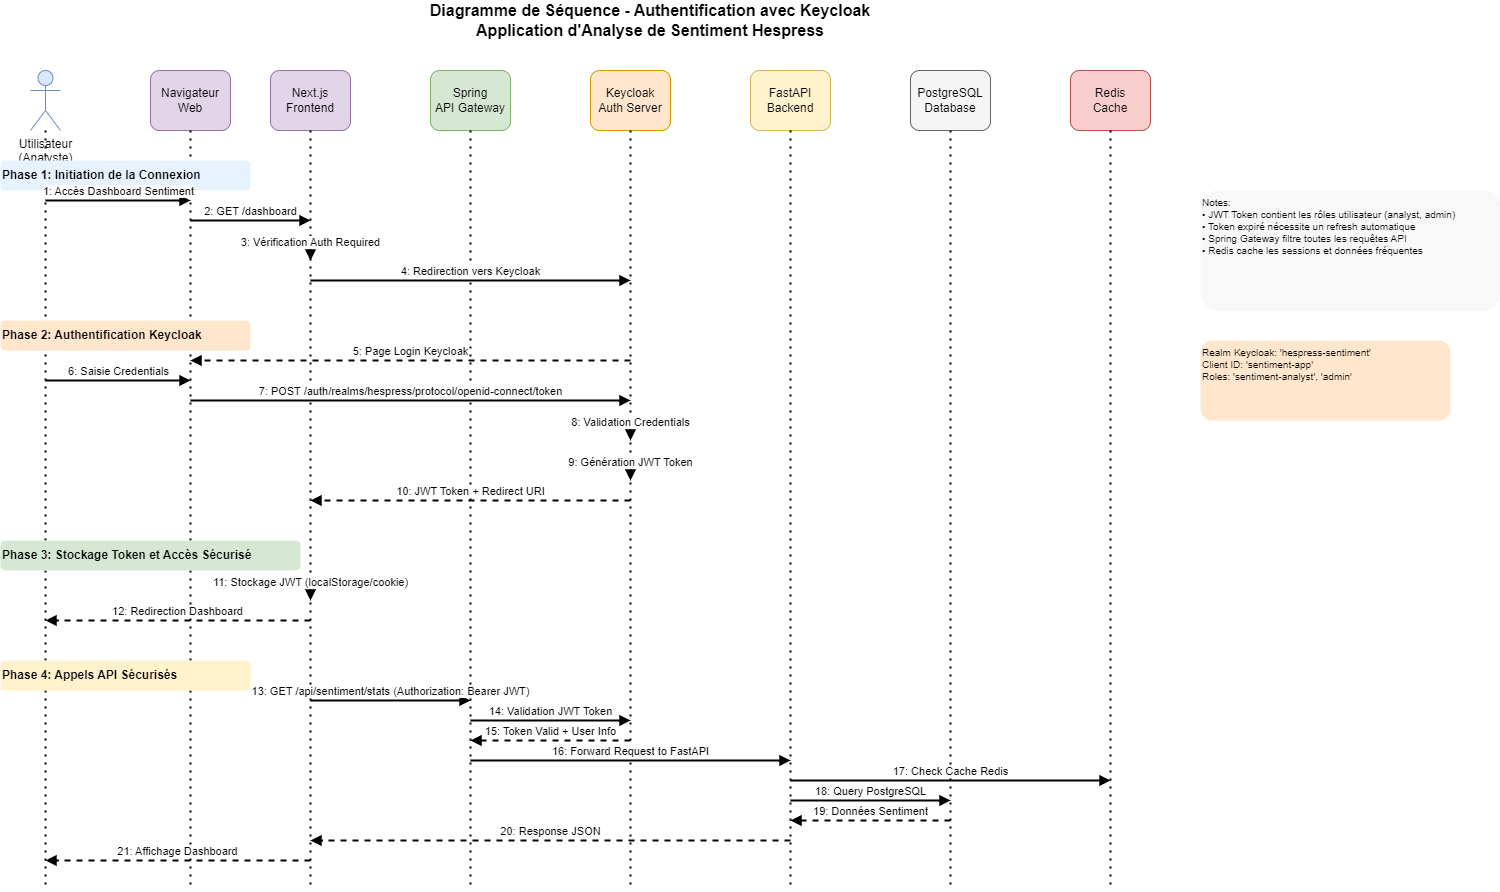
\includegraphics[ width=\textwidth]{assets/images/sprint1-sequence.png}
\caption{Diagramme de sequence pour l'authentification Keycloak}
\label{fig:seq-auth}
\end{figure}
\section{Gestion des Erreurs et Resilience}

\subsection{Strategies de Gestion d'Erreurs}

L'application implemente plusieurs mecanismes pour assurer la resilience :

\begin{itemize}
    \item \textbf{Circuit Breaker} : Protection contre la cascade de pannes
    \item \textbf{Retry Logic} : Nouvelle tentative automatique en cas d'echec temporaire
    \item \textbf{Timeout Management} : Gestion des timeouts pour eviter les blocages
    \item \textbf{Graceful Degradation} : Fonctionnement degrade en cas de panne partielle
\end{itemize}

\subsection{Monitoring et Alertes}

\begin{itemize}
    \item \textbf{Health Checks} : Verification automatique de l'etat des services
    \item \textbf{Metriques personnalisees} : Suivi des performances d'analyse
    \item \textbf{Alertes proactives} : Notification en cas de deviation des metriques
    \item \textbf{Logging structure} : Logs JSON pour faciliter l'analyse
\end{itemize}

\section{Conclusion}

Cette etude technique a detaille l'architecture des microservices de l'application d'analyse de sentiments, les technologies choisies, et les interactions entre les differents services. L'approche microservices, combinee a l'utilisation de technologies modernes comme Next.js, FastAPI, Keycloak et Spring Gateway, assure une application modulaire, securisee, et facilement scalable.

L'integration du modele cardiffnlp/twitter-xlm-roberta-base-sentiment permet une analyse precise et multilingue des sentiments, tandis que l'utilisation de Selenium pour le web scraping automatise la collecte de donnees. Les choix de conception visent a offrir une experience utilisateur optimale tout en garantissant la performance, la securite et la fiabilite de l'application d'analyse de sentiments.

Cette architecture technique solide constitue la fondation necessaire pour le deploiement et l'exploitation d'un systeme d'analyse de sentiments robuste et evolutif, capable de traiter efficacement les commentaires d'Hespress et de fournir des insights precieux sur les opinions publiques.
